\documentclass[border=8pt]{article}
\usepackage[paperwidth=180mm,paperheight=55mm,margin=0mm]{geometry}
\usepackage{xcolor}
\usepackage{tikz}
\usetikzlibrary{arrows.meta,positioning}
\definecolor{navy}{HTML}{18334C}
\definecolor{soft}{HTML}{F3F5F6}
\tikzset{box/.style={draw=navy,line width=.7pt,rounded corners=2pt,fill=soft,align=center,font=\sffamily\small,minimum height=12mm,text width=30mm,inner sep=3mm},arr/.style={-{Stealth[length=2.3mm]},line width=.9pt,draw=navy}}
\pagestyle{empty}
\begin{document}
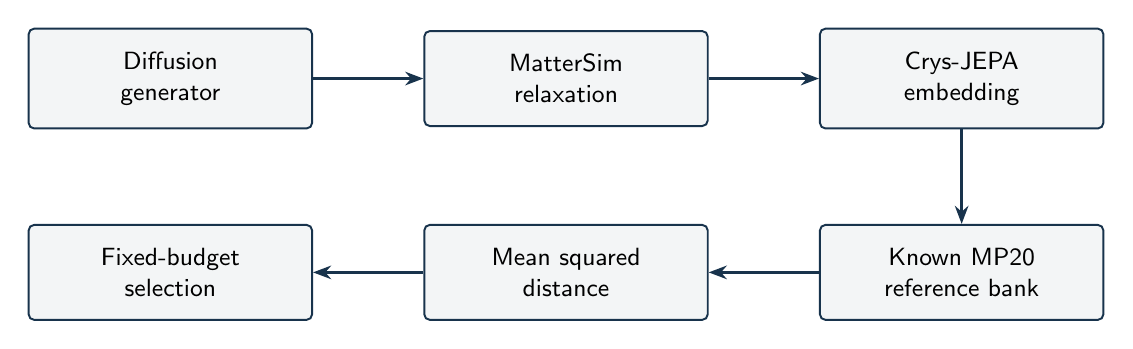
\begin{tikzpicture}[node distance=12mm and 14mm]
\node[box] (gen) {Diffusion\\generator};
\node[box,right=of gen] (rel) {MatterSim\\relaxation};
\node[box,right=of rel] (enc) {Crys-JEPA\\embedding};
\node[box,below=of enc] (refs) {Known MP20\\reference bank};
\node[box,left=of refs] (score) {Mean squared\\distance};
\node[box,left=of score] (select) {Fixed-budget\\selection};
\draw[arr] (gen)--(rel);
\draw[arr] (rel)--(enc);
\draw[arr] (enc)--(refs);
\draw[arr] (refs)--(score);
\draw[arr] (score)--(select);
\end{tikzpicture}
\end{document}
